% \documentclass[12pt,a4paper,openany, ]{book} %el comando "openany" sirve que cuando se hace un Chapter, dejará una hoja en blanco.
\documentclass[12pt,letterpaper]{book}
\usepackage[ruled,vlined]{algorithm2e}
\usepackage{tabularx}
\usepackage{longtable}
%\usepackage{threeparttable} <--
\usepackage{textcomp}
\usepackage[utf8]{inputenc}
\usepackage[T1]{fontenc}

\usepackage{tgtermes} % times font

\usepackage[spanish,es-tabla]{babel}
\usepackage{amsmath}
\usepackage{amsfonts}
\usepackage{amssymb}
\usepackage{graphicx}
\usepackage{subfig}
\usepackage{wasysym}
\usepackage{lscape}
\usepackage[colorlinks=true, linkcolor=black,
citecolor=black, urlcolor=black,hidelinks]{hyperref}
\usepackage{float}
\usepackage{booktabs}
\usepackage{setspace} %por si el titulo es mas largo y el interlineado
\usepackage{xcolor} %para darle color a las lineas del titulo.
\usepackage{lipsum} %crea texto ficticio del texto Lorem Ipsum
%\definecolor{azul}{rgb}{0.17, 0.4, 0.69} %definir color de lineas.
% \usepackage{natbib}
%\usepackage[left=2.54cm,top=2.54cm,right=2.54cm,,bottom=2.54cm]{geometry} %para cambiar la configuracion de las medidas a APA se usa "Control + R".

\usepackage[left=3cm,top=3cm,right=3cm,,bottom=4cm]{geometry}

\usepackage[justification=centering]{caption}
% Reducimos el espacio debajo de las figuras
\captionsetup{belowskip=0pt}

\newcommand{\grad}{$^{\circ}$}
\renewcommand{\baselinestretch}{1.5} %interlineado 1.5

\usepackage{csquotes}
\usepackage[backend=biber,natbib,url=false,doi=false,style=apa,maxcitenames=5]{biblatex}

% Cuando el idioma es otro "et al." cambia, con este comando se fuerza a si o si usar "et al."
\DefineBibliographyStrings{spanish}{%
  andothers = {et\addabbrvspace al\adddot}
}
\addbibresource{capitulos/biblio.bib}

% SE ELIMINA LA PALABRA "CAPÍTULO" DEL TÍTULO
\usepackage{titlesec}

% Capítulos sin la palabra "Capítulo "
\titleformat{\chapter}
  {\normalsize\bfseries}{\thechapter.}{0.5em}{}
%   \titlespacing*{\chapter}{0pt}{2pt}{2pt}
\titlespacing*{\chapter}{0pt}{0pt}{0pt}[0pt]
% \titlespacing*{\chapter}{0pt}{3.5ex plus 1ex minus .2ex}{2.3ex plus .2ex}

% Cambiamos el tamaño de las secciones
\titleformat{\section}
  {\normalfont\normalsize\bfseries}{\thesection.}{0.5em}{}
\titleformat{\subsection}
  {\normalfont\normalsize\bfseries}{\thesubsection.}{0.5em}{}

% SE ELIMINA LA CABECERA DE LAS HOJAS Y LA NUMERACIÓN ES ABAJO
\usepackage{fancyhdr}
\fancyhf{}
\renewcommand\headrulewidth{0pt}
% \fancyfoot[RO, LE]{\thepage}
% \fancyfoot[C]{\thepage}
% SE ENUMERA A LA DERECHA
\fancyfoot[R]{\thepage}
% SE REDEFINE EL ESTILO PARA ENUMERAR LAS PÁGINAS DE CAPÍTULO A LA DERECHA
\pagestyle{fancy}
\fancypagestyle{plain}{%
    \renewcommand{\headrulewidth}{0pt}%
    \fancyhf{}%
    \fancyfoot[R]{\thepage}%
}

% \renewcommand{\contentsname}{Índice}

% Remove indentation for section, subsection, and paragraph in TOC
\usepackage[subfigure]{tocloft}
% \setlength{\cftpartindent}{0em}
% \setlength{\cftchapindent}{0em}
\setlength{\cftsecindent}{0em}
\setlength{\cftsubsecindent}{0em}
\setlength{\cftsubsubsecindent}{0em}
% \setlength{\cftsubsubsecindent}{3em}
%\cftsetindents{section}{0em}{2.3em}
%\cftsetindents{subsection}{0em}{3.2em}
\cftsetindents{paragraph}{0em}{3.7em}

% Redefinir el comando \paragraph para que no aparezca en el índice
%\usepackage{titlesec}
%\titleformat{\paragraph}[runin]{\normalfont\normalsize\bfseries}{\theparagraph}{1em}{}
%\titlespacing*{\paragraph}{0pt}{3.25ex plus 1ex minus .2ex}{1em}

%\usepackage{etoolbox}

% Redefinir el comando \paragraph para que no aparezca en el índice
%\makeatletter
%\patchcmd{\paragraph}{\addcontentsline{toc}{paragraph}{\theparagraph}}{}{}{}
%\makeatother

\usepackage{enumitem}
\setcounter{tocdepth}{4}
\setcounter{secnumdepth}{4}

% https://tex.stackexchange.com/questions/395856/switching-tocdepth-in-the-middle-of-a-document
\newcommand{\changelocaltocdepth}[1]{%
  \addtocontents{toc}{\protect\setcounter{tocdepth}{#1}}%
  \setcounter{tocdepth}{#1}%
}

\renewcommand*{\listalgorithmcfname}{Lista de Algoritmos}
\renewcommand*{\algorithmcfname}{Algoritmo}
\renewcommand*{\algorithmautorefname}{algoritmo}
\SetKwInput{KwData}{Requiere}

\makeatletter
\patchcmd{\chapter}{\if@openright\cleardoublepage\else\clearpage\fi}{}{}{}
\makeatother

% Contar las figuras sin el capítulo
\usepackage{chngcntr}
\counterwithout{figure}{chapter}

%\usepackage{tikz}
%\usetikzlibrary{shapes.geometric, arrows}
% Definición del estilo 'process'
%\tikzstyle{startstop} = [rectangle, rounded corners, minimum width=3cm, minimum height=1cm,text centered, draw=black, fill=red!30]
%\tikzstyle{process} = [rectangle, minimum width=3cm, minimum height=1cm, text centered, draw=black, fill=blue!30]
%\tikzstyle{arrow} = [thick,->,>=stealth]

% Editando el titulo del indice
\addto\captionsspanish{% Replace "spanish" with the language you use
  \renewcommand{\contentsname}%
    {\fontsize{16}{20}\selectfont ÍNDICE}
}
% quitando espacio del titulo del indice
\setlength{\cftbeforetoctitleskip}{-1em}
\setlength{\cftaftertoctitleskip}{1em}

% Quitando el identado en cada parrafo
\setlength\parindent{0pt}

% Espaciado entre parrafos
\setlength{\parskip}{0.5em}

%\usepackage[smartEllipses]{markdown}

\usepackage{blindtext}

\begin{document}
    %FRONTMATTER
    %---------------------------------------------------
    \frontmatter %numeros romanos
    \begin{titlepage} %este titlepage sirve para poder realizar el titulo de una pagina, la caratula de un libro y no se enumere esta.
	\begin{center}
	    {\fontsize{20}{20}\selectfont \textbf{UNIVERSIDAD MAYOR DE SAN ANDRÉS}}
		{\fontsize{16}{16}\selectfont \textbf{FACULTAD DE CIENCIAS PURAS Y NATURALES\\
		CARRERA DE INFORMÁTICA}}
		%\vspace{1mm}
		
		
\includegraphics[scale=0.093]{imagenes/logo-umsa.png}
		%\vspace{1mm}
		
		{\fontsize{16}{20}\selectfont \textbf{TESIS DE GRADO}}\\
		%\vspace{2mm}
		
        {\fontsize{16}{18}\selectfont \textbf{APLICACIÓN WEB PARA INCREMENTAR EL RENDIMIENTO EN CONCURSOS DE PROGRAMACIÓN COMPETITIVA TIPO ICPC}}
		
		{\fontsize{12}{12}\selectfont\textbf{Tesis de Grado para obtener el Título de Licenciatura en Informática Mención Ingeniería de Sistemas Informáticos}}
 		%\vspace{2mm}
		
		{\fontsize{16}{16}\selectfont\textbf{POR: OSCAR GAUSS CARVAJAL YUCRA}}\\
    	{\fontsize{14}{14}\selectfont\textbf{TUTOR METODOLÓGICO: MS.C. GROVER ALEX RODRIGUEZ RAMÍREZ\\
    	ASESOR: M.SC. JORGE HUMBERTO TERÁN POMIER}}
		%\vspace{2mm}
		 
		\textbf{LA PAZ - BOLIVIA\\
		Abril, 2024}
	\end{center}
\end{titlepage}
% 	

	\begin{flushleft}
	\large {\textbf{Personal Investigador:}}
	\end{flushleft}

		\vspace{1.25cm}
%--------------------------------------------------------------
	\begin{flushleft}
	\rule{70mm}{0.2mm} \hspace{0.3cm} \rule{83mm}{0.2mm}\\
	\large  {\textbf{Niño Mocarro Jorge Vicente}} \hspace{0.36cm} \large {\textbf{Llenque Sánchez, Walther Enrique}}\\ 					\hspace{2.20cm}\textsc{Estudiante} \hspace{5cm}\textsc{Estudiante}
	\end{flushleft}
%--------------------------------------------------------------
		\vspace{2cm} %Cedo 2cm de espacio horizontal para seguir escribiendo.
		
		\begin{center}
		\rule{70mm}{0.2mm}\\
		\large{\textbf{<Nombre del Asesor>}}\\
		\textsc{Asesor}
		\end{center}
	\vspace{0.35cm}
%--------------------------------------------------------------
\begin{flushleft}
\large{\textbf{Aprobado por el Jurado:}}
\end{flushleft}

	\vspace{1.2cm}
%--------------------------------------------------------------
	\begin{flushleft}
	\hspace{1cm} \rule{60mm}{0.2mm} \hspace{2.25cm} \rule{50mm}{0.2mm}\\
	\hspace{2.3cm} \large{\textbf{<Presidente>}} \hspace{4.45cm} \large{\textbf{<Secretario>}}\\ 
	\end{flushleft}
	\vspace{1.15cm}
%------------------
	\begin{center}
		\rule{60mm}{0.2mm}\\
		\large{\textbf{<Vocal>}}\\
		\end{center}
	\vspace{0.5cm}
%--------------------------------------------------------
\begin{center}
	\begin{tabular}{|c|c|c|c|}
	\hline 
	 & \large{Apellidos y Nombres} & \large{Correo Electrónico} & \large{Teléfono} \\ 
	\hline 
	\large{Presidente} & • & • & • \\ 
	\hline 
	\large{Secretario} & • & • & • \\ 
	\hline 
	\large{Vocal} & • & • & • \\ 
	\hline 
	\end{tabular} 
\end{center}
%--------------------------------------------------------------	
$\ $
\thispagestyle{empty} % para que no se numere esta pagina
% 	\chapter*{Agradecimientos}
	
	
    %ÍNDICE O TABLA DE CONTENIDO-------------------
    \tableofcontents
    \setcounter{page}{0}
    %\cleardoublepage
% 	\addcontentsline{toc}{chapter}{Lista de figuras} % para 						que aparezca en el indice de contenidos
% 	\listoffigures % indice de figuras
	%\cleardoublepage
% 	\addcontentsline{toc}{chapter}{Lista de tablas} % para que 						aparezca en el indice de contenidos
% 	\listoftables % indice de tablas
	
	 % si no queremos que añada la palabra "Capitulo"
% 	\addcontentsline{toc}{chapter}{INTRODUCCIÓN} % si queremos que aparezca en el índice
    %\markboth{AGRADECIMIENTOS}{AGRADECIMIENTOS} % encabezado
    
    %MAINMATTER
    %--------------------------------------------------	
    \mainmatter %numeros arabicos.
    
    % \begingroup
    % \renewcommand{\cleardoublepage}{}
    % \renewcommand{\clearpage}{}
    
    \raggedbottom
    
    % \thispagestyle{empty}

    \chapter{MARCO REFERENCIAL}

\section{INTRODUCCIÓN}

Los concursantes que participan en las competencias de programación competitiva son principalmente alumnos con experiencia en programación autodidacta que vienen preparándose con recursos en su totalidad o mayoría en ingles.

% La programación de computadoras es el proceso de desarrollar e implementar varios conjuntos de instrucciones para permitir que una computadora realice una determinada tarea, resuelva problemas y proporcione interactividad humana. Estas instrucciones (códigos fuente que están escritos en un lenguaje de programación) se consideran programas de computadora y ayudan a que la computadora funcione sin problemas \citep{Balanskat-Engelhardt}.

El pensamiento computacional generalmente es asociado con la programación , pero es mucho más que eso, implica resolver problemas, diseñar sistemas y comprender el comportamiento humano recurriendo a los conceptos fundamentales de la informática. Pensar como un informático significa más que ser capaz de programar una computadora. Requiere la capacidad de abstraer y, por lo tanto, pensar en múltiples niveles de abstracción \citep{Wing}.

La programación competitiva es considerado un deporte mental, generalmente es practicado en línea y en algunas ocasiones de forma presencial en el que a cada equipo se le otorga un solo equipo para concursar. Existen competencias en donde se puede participar de forma individual y existen otras en las que se participa en equipos, generalmente en equipos de 3 integrantes. En este tipo de concursos gana aquel equipo que resuelve la mayor cantidad de problemas planteados en el concurso, si hay equipos que tiene la misma cantidad de problemas resueltos entonces gana aquel que los resolvió en menos tiempo. 

Cada persona y equipo que participan en estos concursos de programación competitiva emplean diversos métodos y estrategias para prepararse y entrenar con el objetivo de quedar primeros o en unos de las primeras posiciones en la tabla final del ranking general del concurso para. Para ello muchos estudiantes optan por asistir a los campamentos de programación competitiva que se realizan entre 1 o 2 semanas donde entrenan intensamente el pensamiento computacional y el diseño de algoritmos.

El presente trabajo plantea mejorar el rendimiento de los participantes en los concursos de programación competitiva con formato ICPC mediante una plataforma web de entrenamiento individual y por equipos de concursantes.

\section{PROBLEMA}

\subsection{ANTECEDENTES}

Existen varias iniciativas para apoyar a las personas en la programación de aprendizaje. Por ejemplo, los concursos de programación son una buena motivación para que las personas aprendan y mejoren sus habilidades.
Sin embargo, los concursantes deben aprender por sí mismos si no se organizan entrenamientos. Los concursos como las olimpiadas también apuntan a la excelencia, excluyendo a las personas menos calificadas. Un aspecto positivo de los concursos son las discusiones que desencadena entre los concursantes, especialmente para los concursos no en línea \citep{Combéfis-Saint_Marcq}.

\subsubsection{PLATAFORMAS WEB DE PROGRAMACIÓN}

\begin{itemize}
    \item visualgo: VisuAlgo fue conceptualizado en 2011 por el Dr. Steven Halim como una herramienta para ayudar a sus estudiantes a comprender mejor las estructuras de datos y los algoritmos, permitiéndoles aprender los conceptos básicos por su cuenta y a su propio ritmo. VisuAlgo contiene muchos algoritmos avanzados que se analizan en el libro del Dr. Steven Halim (Programación competitiva, en coautoría con su hermano, el Dr. Félix Halim) y más allá. Inicialmente fue diseñado para estudiantes de la Universidad Nacional de Singapur (NUS) que toman varias clases de estructura de datos y algoritmos (por ejemplo, CS1010, CS1020, CS2010, CS2020, CS3230 y CS3230), esta plataforma fue adoptaba por la comunidad de programación competitiva. VisuAlgo no está diseñado para funcionar bien en pantallas táctiles pequeñas (por ejemplo, teléfonos inteligentes) desde el principio debido a la necesidad de satisfacer muchas visualizaciones de algoritmos complejos que requieren muchos píxeles y gestos de hacer clic y arrastrar para interactuar. La resolución mínima de pantalla para una experiencia de usuario respetable es 1024x768 y solo la página de destino es relativamente amigable para dispositivos móviles \citep{visualgo}.
    \item algoexpert.io: Es una plataforma web para prepararse en programación y algoritmia, si bien en esta plataforma se puede encontrar material de muy buena calidad sobre algoritmia esta no esta enfocada a programación competitiva si no a pruebas de entrevistas de trabajo. Para acceder a los recursos que te ofrece la plataforma se debe contar con una suscripción anual de paga que puede ir desde los 60 dolares americanos hasta los 160 dolares americanos por año.
    \item Coursera: Coursera fue fundada por Daphne Koller y Andrew Ng con la visión de proporcionar experiencias de aprendizaje transformadoras para cualquier persona, en cualquier lugar. Ahora es una plataforma de aprendizaje en línea para la educación superior, donde 66 millones de estudiantes de todo el mundo vienen a aprender habilidades del futuro \citep{coursera}. 
    \item platzi: John Freddy Vega y Christian Van Der Henst describen a Platzi como educación online efectiva, Platzi es una de las primeras plataformas que tiene contenidos de tecnología en español enfocado para personas de Latinoamerica. Si bien todo los recursos están en español no se encuentra material especializado en programación competitiva.
\end{itemize}

\subsubsection{TRABAJOS SIMILARES}

\begin{itemize}
    \item [\textbullet]
    \begin{itemize}[nosep]
        \item[] \textbf{Título:} Método conectivo bajo presión v-bloom para el aprendizaje de programación competitiva orientada a participantes de la olimpiada boliviana de informática 
        \item[] \textbf{Autor:} Quispe Valdez, Saúl
        \item[] \textbf{Institución:} Universidad Mayor de San Andrés
        \item[] \textbf{Gestión:} 2017
        \item[] \textbf{Descripción:} Esta investigación trabaja sobre el tema de tecnología informática en el ámbito educativo. Inicialmente se presenta un sustento teórico para luego diseñar el denominado método conectivo bajo presión V-Bloom, orientado a la enseñanza aprendizaje de programación competitiva para estudiantes de nivel escolar con edades comprendidas 11 y 15 años. En una segunda instancia se prueba la validez del mismo en 3 evaluaciones correspondientes a las 4 etapas de la 7ma Olimpiada Científica Estudiantil Plurinacional Boliviana 2017 en el área de Informática (Nivel 2). Finalmente, se proporciona una interpretación de los resultados obtenidos y se presentan las conclusiones del trabajo.
    \end{itemize}

    \item [\textbullet]
    \begin{itemize}[nosep]
        \item[] \textbf{Título:} Tutor inteligente para el proceso de aprendizaje en algoritmos y programación en el lenguaje java
        \item[] \textbf{Autor:} Espejo Cuba, Jose Gonzalo
        \item[] \textbf{Institución:} Universidad Mayor de San Andrés
        \item[] \textbf{Gestión:} 2015
        \item[] \textbf{Descripción:} El presente trabajo aborda la formación de estudiantes principiantes en el área de algoritmos y programación en el lenguaje Java desarrollando un tutor inteligente que mejora el proceso de aprendizaje de algoritmos y programación en el lenguaje Java siendo este uno de los tantos lenguajes de programación, elegido por ser portable, gratuito, se pueden desarrollar programas incluso para celulares y cada día se desarrollan nuevas herramientas.
    \end{itemize}
\end{itemize}
\subsection{PLANTEAMIENTO DEL PROBLEMA}

%Cuando se enseña en las escuelas secundarias, los profesores de otras disciplinas, como las matemáticas o la física, se hacen cargo de la informática. La misma situación ocurre en muchos otros países. Los profesores no siempre tienen la experiencia adecuada para poder enseñar ciencias de la computación. A veces incluso se les pide que enseñen ciencias de la computación, pero simplemente no saben qué hacer \citep{Combéfis-Saint_Marcq}.

\subsubsection{PROBLEMA CENTRAL}
¿Cómo incrementar el rendimiento en estudiantes para los concursos de programación competitiva del tipo ICPC? 

\subsubsection{PROBLEMAS SECUNDARIOS}
\begin{itemize}[nosep]
    \item[\textbullet] Los recursos necesarios para aprenden algoritmos, paradigmas de programación necesarios en competencias de programación competitiva debe ser seleccionado de varios plataformas y varios documentos y/o textos ocasionando que el entrenamiento sea lento.
    \item[\textbullet] La comunidad de programación competitiva en Bolivia es limitada debido a esto los estudiantes no desconocen o no se motivan para participar en estos tipo de concursos.
    \item[\textbullet] Los contenidos que se debe conocer y aprender para lograr una buena posición en estos tipos de concursos son amplios, por este motivo los equipos tienen dificultades en organizar su plan de estudio y entrenamiento.
\end{itemize}

\subsection{FORMULACIÓN DEL PROBLEMA}
\section{OBJETIVOS}

\subsection{OBJETIVO GENERAL}
Desarrollar una aplicación web de entrenamiento para estudiantes de los concursos de programación competitiva del tipo ICPC.

\subsection{OBJETIVOS ESPECÍFICOS}
\begin{itemize}[nosep]
    \item[\textbullet] Brindar a los estudiantes herramientas para el entrenamiento en algoritmos y paradigmas de programación. 
    \item[\textbullet] Fomentar la participación en concursos de programación del tipo ICPC. 
    \item[\textbullet] Brindar a los estudiantes una herramienta virtual para la organización y planificación de su plan de estudio.
\end{itemize}
\section{HIPÓTESIS}
El desarrollo de una aplicación web de entrenamiento mejora el rendimiento de los estudiantes, para los concursos de programación competitiva del tipo ICPC en un 35\%.

\subsection{OPERACIONALIZACIÓN DE VARIABLES}
Analizando la hipótesis de la investigación, se identificó las variables:

\begin{center}
    \begin{tabular}{|c|c|}
        \hline
        \textbf{Variable} & \textbf{Tipo} \\
        \hline
        Aplicación web de entrenamiento & Independiente \\
        \hline
        Rendimiento de equipos en concursos de programación competitiva & Dependiente \\
        \hline
        Tecnologías web & Interviniente\\
        \hline
    \end{tabular}\\
    \vspace{2mm}
    \textbf{Fuente:} Elaboración propia
\end{center}
\section{JUSTIFICACIÓN}
    %\subsection{JUSTIFICACIÓN TECNOLÓGICA}
    \subsection{JUSTIFICACIÓN SOCIAL}
    Visto los problemas observados en concursantes al tener que organizarse, buscar recursos incluso buscar un entrenador y la poca participación de estudiantes por los problemas descritos el presente trabajo propone realizar una plataforma web de entrenamiento para estos tipos de concursos ayudando y acelerando el proceso de entrenamiento.
    \subsection{JUSTIFICACIÓN ECONÓMICA}
    La implementación de una plataforma con el fin de entrenar a los participantes de concursos de programación competitiva reduce los costos sin tener que tomar clases particulares en instituciones o cursos en linea de paga, evita la compra de libros de programación, minimiza el tiempo de organización y búsqueda de material en internet.
    \subsection{JUSTIFICACIÓN CIENTÍFICA}
    Para el uso de la plataforma no será necesario tener que instalar software extra más que un navegador web así el presente trabajo  abrirá un camino a los estudiantes y a la población en linea a la investigación sobre las formas de entrenamiento vía web.
\section{ALCANCES Y LÍMITES}
    \subsection{ALCANCES}
    El presente trabajo contemplara una gran parte del conocimiento requerido para participar en los concursos de programación competitiva tipo ICPC. Se establecerá una comunicación entre el competidor - plataforma y equipo - plataforma y en algunos casos entrenador - plataforma - equipo, de esta manera conseguimos acelerar el entrenamiento y mejorando el rendimiento de los equipos en competencias.
    \subsection{LÍMITES}
    La plataforma web solo sera podrá ser usada para el entrenamiento en competencias formato ICPC.
    La plataforma web sera orientada para estudiantes universitarios y no así para estudiantes de primaria o secundaria.
    
    La plataforma web necesitará estar conectado a internet.
    Los recursos de la plataforma estarán disponibles solo en el idioma español, incluyendo las opciones de visualización.
    
    
\section{APORTES}
    \subsection{PRÁCTICO}
    La plataforma web registra el entrenamiento de los concursantes y equipos los mismos podrán obtener los registros de su desempeño en la plataforma web.
    El tutor interactivo aceptara estudiantes de distintas edades y de distintos niveles en programación competitiva. La plataforma web podrá ser utilizado en cualquier horario que sea mas conveniente para el concursante y para el equipo.  
    \subsection{TEÓRICO}
   El presente trabajo pretende contribuir en el área del aprendizaje con el desarrollo de una plataforma web aprovechando las nuevas tecnologías, con el fin de que la plataforma pueda entrenar a estudiantes universitarios en un mejor tiempo y de manera eficaz.
\section{METODOLOGÍA}
El tipo de investigación es exploratorio - descriptivo, los estudios exploratorios en una investigación se realizan cuando el objetivo a examinar es poco estudiado, del cual se desprenderán muchas dudas y centra el estudio en fenómenos novedosos.

Para la parte de desarrollo se hará uso de la metodología de desarrollo ágil SCRUM ya que nos permite agilizar la estructura del desarrollo del proyecto en iteraciones cortas de tiempo.

Para la parte de la metodología de modelado web se utilizara ya que esta proporciona especificaciones gráficas, formales, incorporadas en un proceso de diseño completo, que puede ser asistido por herramientas de diseño visual.

Para el desarrollo de la plataforma se usarán como lenguaje principal JavaScript para la aplicación Web junto con la librería React. Para la parte del backend se usará NodeJs con una base de datos dentro del entorno de MongoDB.

    %\newpage
\chapter{MARCO TEÓRICO}

En este capítulo se explicará en qué consisten los concursos de programación para tener concretar una idea clara y la importancia de los jueces en línea en ese campo, después se mencionarán los jueces en línea con más popularidad a nivel internacional y algunas plataformas donde se puede encontrar recursos aunque poco enfocados a programación competitiva.

\section{PROGRAMACIÓN COMPETITIVA}

Hay muchos tipos diferentes de concursos de programación en línea. El objetivo principal de tales concursos es permitir que concursantes o equipos de concursantes compitan. Los concursos pueden ser de muchos tipos diferentes: encontrar el algoritmo más eficiente, modelar un problema desafiante y escribir un programa para resolverlo, desarrollar un algoritmo de inteligencia artificial (IA) que se ejecute contra IA de otros concursantes. Además del concurso en sí y su objetivo principal, participar en dichos concursos también es una forma para que los concursantes aprendan y mejoren sus propias habilidades. Cuanto mejor y más relevante sea el apoyo al concursante y la retroalimentación recibida, más su aprendizaje será de buena calidad. Por ejemplo, proporcionar a los concursantes la solución correcta anotada con explicaciones al final del concurso, o permitirles participar en equipos puede mejorar su aprendizaje \citep{Combéfis-Wautelet}.

\subsection{INICIOS DE LOS CONCURSOS DE PROGRAMACIÓN COMPETITIVA}
La Competencia Internacional de Programación Universitaria (ICPC por sus siglas en inglés) se inician en 1970, cuando los pioneros de Alpha Chapter de la “Sociedad de honor de ciencias en computación” (UPE) presentaron la primera competencia de este estilo. La iniciativa se propagó rápidamente hacia los Estados Unidos y Canadá como un programa de innovación para incrementar ambición, aptitud de resolución de problemas, y la oportunidad para estudiantes fuertes en el campo de la computación \citep{icpc-glogal}.

Con el tiempo, el concurso se convirtió en una competencia de varios niveles con la primera ronda de campeonato realizada en 1977; desde entonces el concurso se ha expandido a una colaboración mundial de universidades que albergan competencias regionales que hacen avanzar a los equipos a la ronda anual de campeonato mundial, el ICPC World Finales \citep{icpc-glogal}.

El concurso internacional de programación universitaria, \textit{International Collegiate Programming Contest} (ICPC), es el concurso de programación más antiguo, más grande y más prestigioso del mundo. La ICPC tiene sus raíces en 1970, cuando los pioneros del Capítulo Alpha de la Sociedad de Honor de Ciencias de la Computación de la UPE organizaron la primera competencia. La iniciativa se extendió rápidamente dentro de los Estados Unidos y Canadá como un programa innovador para aumentar la ambición, la capacidad de resolución de problemas y las oportunidades de los estudiantes más fuertes en el campo de la informática. Con el tiempo, el concurso se convirtió en una competencia de varios niveles con la primera ronda de campeonato realizada en 1977. Desde entonces, el concurso se ha expandido a una colaboración mundial de universidades que organizan competiciones regionales que llevan a los equipos a la ronda anual de campeonato mundial, la ICPC World Final \citep{icpc-glogal}.

\begin{figure}[H]
    \centering
    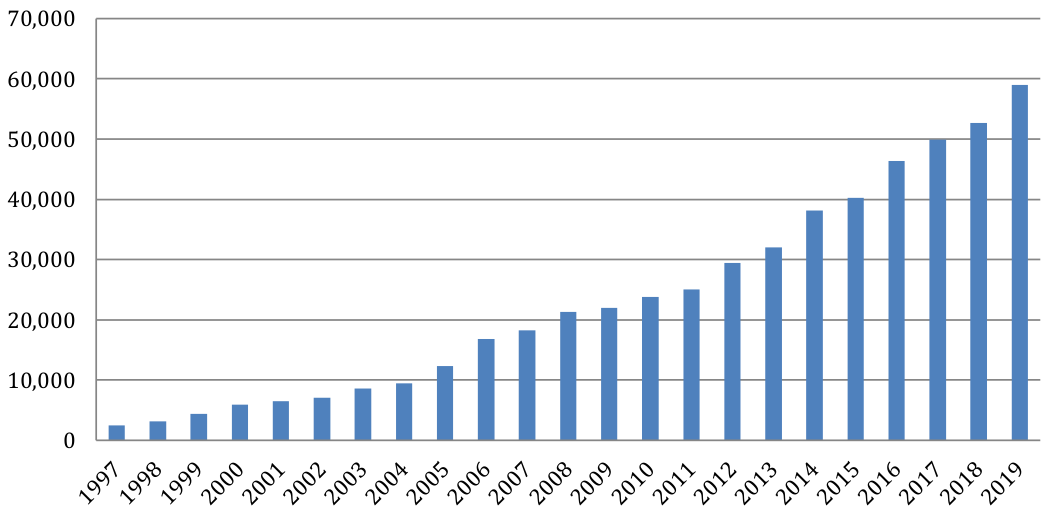
\includegraphics[scale=0.7]{imagenes/ICPC_student_participation.png}
    \caption{Participación de estudiantes en la ICPC\\ Fuente: \citep{icpc-glogal}}
\end{figure}

El concurso fomenta la creatividad, el trabajo en equipo y la innovación en la creación de nuevos programas de software, y permite a los estudiantes probar su capacidad para desempeñarse bajo presión. El concurso ha elevado las aspiraciones y el rendimiento de generaciones de solucionadores de problemas del mundo en ciencias de la computación e ingeniería. La ICPC presenta varios niveles de competencia:  

\begin{itemize}
    \item Campeonato Interno por Universidad
    \item Campeonato Departamental/Estatal. 
    \item Campeonato Nacional. 
    \item Campeonato Regional.
    \item Final Mundial. 
\end{itemize}

Los participantes conforman equipos de tres personas, cada equipo representa a su universidad y país respectivamente. El concurso dura cinco horas, tiempo en que los estudiantes deben resolver de ocho a trece problemas algorítmicos. Un equipo es ganador cuando éste resuelve la mayor cantidad de problemas en el menor tiempo de penalización (Wasik et al. 2018).

\subsection{PROGRAMACIÓN COMPETITIVA EN LATINOAMERICA}

En Bolivia también se llevan a cabo las competencias de programación competitiva, entre estos tenemos:
\begin{itemize}
    \item Olimpiadas Bolivianas en Informática (OBI): Se fundaron el año 2011, estas Olimpiadas están orientadas a niños de tercero hasta sexto de secundaria donde los primeros veinte clasificados pasan a formar un equipo que después de un año de capacitación compiten para los cuatro puestos para representar a Bolivia en la competencia \textit{International Olympiad in Informatics} (IOI)
    \item Red de programación competitiva (RPC): Se fundó hace siete años en Colombia, en el cual, cualquier persona o grupos de tres personas pueden inscribirse libremente y participar, la evaluación es de la misma modalidad de la ICPC. Cada una de las universidades bolivianas tienen una sede dentro del concurso, suele llevarse a cabo en tiempo real junto con otras universidades latinoamericanas. Este concurso se realiza cada 3 semanas aproximadamente.
    \item Torne Argentino de Programación (TAP): Es una competencia por equipos de 3 estudiantes de la misma institución de educación superior de Argentina. La competencia tiene 5 horas de duración, en las que cada equipo deberá resolver un conjunto de problemas algorítmicos, creando un programa que solucione cada problema, la evaluación es de la misma modalidad de la ICPC, este concurso se celebra cada año y sirve como un clasificatorio para los concursantes Argentinos a la fase Latinoamericana de Programación.
\end{itemize}

\subsection{JUEZ}

La clave principal para este tipo de concursos anteriormente mencionados es el sistema que verifica automáticamente la corrección de las soluciones presentadas por los participantes, también verifica que la solución no exceda los límites de utilización de recursos (como el tiempo y la memoria). Según la evaluación realizada, se calcula la clasificación en línea de todos los participantes presentado en tiempo real durante el desarrollo de un concurso.

El término juez fue introducido por primera vez el año 2001 por Kurnia, Lim y Cheang como una plataforma en línea que está inspirada tanto para las competencias de programación como para la educación. Kurnia, Lim y Cheang le dan forma a esta definición como una plataforma que puede evaluar automáticamente cualquier programa escrito en cierto lenguaje de programación en tiempo real. \citep{KURNIA2001299}

En general, el objetivo de los sistemas de jueces en línea es evaluar los programas algorítmicos de manera segura, confiable y continua.
A continuación se describe el proceso de evaluación:

1) Envío,

2) Evaluación

3) Puntuación.

Para cada ejecución de caso de prueba de la presentación particular, se verifica si:

1) El proceso de ejecución se realizó sin errores.

2) No se han excedido las limitaciones de recursos específicos del problema.

3) El resultado obtenido cumple con las reglas descritas en la definición del problema (Wasik et al. 2018).

En la actualidad, existen plataformas en línea que comparten desafíos similares a los que se utilizan para las competencias de programación, muchas universidades proveen este tipo de
sistemas para apoyar a sus estudiantes para la preparación de los concursos de programación.
\begin{itemize}
    \item \textit{UVa Online Judge}: Este juez en línea tiene sus inicios en noviembre de 1995, fue desarrollado inicialmente por un estudiante de informática para una competencia de programación que se iba a realizar en la Universidad de Valladolid en España; con el tiempo ese juez llegó a ser perfeccionado y ya no sólo se le utilizaba para las competencias de programación, sino también para el entrenamiento constante de los competidores del mundo ya que éste tenía una gran cantidad de desafíos de programación competitiva. Es el repositorio oficial para los problemas del ICPC , competencias regionales y la de los mundiales de programación (Revilla et al, 2018).
    \item Codeforces: Tiene sus inicios en el año 2010, su fundador es Mike Mirzayanov. Este juez en línea es uno de los más populares a nivel mundial, en un inicio fue preparado para los concursantes de nacionalidad rusa. Su forma de evaluación consiste en dos divisiones según su calificación de Elo, que se actualiza para cada competencia realizada \citep{codeforces}.
    \item SPOJ: Sphere Online Judge, es un juez en línea que tiene diversos desafíos de programación de todo tipo de nivel y se los puede clasificar mediante etiquetas \citep{spoj}.
    \item TopCoder: Es una empresa con comunidad global abierta de diseñadores, desarrolladores, científicos de datos, y programadores competitivos. En programación competitiva, topcoder gira alrededor de una ronda de competencias en su plataforma de juzgamiento SRM cronometrados de 1,5 horas en el que todos los participantes compiten en línea que tratan de resolver el mismo conjunto de problemas tan rápidamente como sea posible. Estos fueron el primer tipo de desafíos en Topcoder \citep{topcoder}.
    \item Codechef: Tiene sus inicios en septiembre de 2009 en Mumbai India. Se creó como una plataforma para ayudar a los programadores a triunfar en el mundo de los algoritmos, la programación de computadoras y los concursos de programación.
    En CodeChef se organiza un concurso de programación a principios de mes y dos desafíos de programación más pequeños a mediados y finales de mes. Esta plataforma también tiene sesiones de capacitación y discusiones relacionadas con algoritmos, búsqueda binaria, tecnicismos como el tamaño de la matriz y los gustos. Y como complemento final, la plataforma tiene varios documentos de algoritmos y debates en foros para ayudar a aquellos que son nuevos en el mundo de la programación de computadoras \citep{codechef}.
\end{itemize}

\section{CONTENIDO EN COMPETENCIAS DE PROGRAMACIÓN COMPETITIVA}
\changelocaltocdepth{2}
\subsection{Introducción}
\subsubsection{Conceptos}
La programación competitiva es una actividad que consiste en resolver problemas algorítmicos bajo ciertas restricciones de tiempo y espacio. Los competidores deben diseñar algoritmos eficientes para solucionar problemas específicos dentro de un tiempo limitado \cite{skiena2008algorithm}.
\paragraph{Lenguaje de Programación}
El lenguaje de programación es una herramienta fundamental para resolver problemas. Los lenguajes más utilizados en la programación competitiva incluyen C++, Java y Python, debido a su eficiencia y versatilidad \cite{stroustrup2013c++}.
\paragraph{Programación Competitiva}
La programación competitiva se basa en la capacidad de diseñar algoritmos eficientes y optimizar el uso de recursos. Es una disciplina que ayuda a mejorar las habilidades de resolución de problemas y el pensamiento lógico \cite{ahmed2020competitive}.
\paragraph{Herramientas}
Existen varias herramientas que facilitan la práctica de la programación competitiva, como compiladores, entornos de desarrollo integrado (IDE) y sistemas de control de versiones \cite{menezes2018tools}.

\subsubsection{Jueces}
Los jueces son plataformas en línea que permiten a los programadores competir y verificar la corrección de sus soluciones. Ejemplos populares incluyen Codeforces, LeetCode y HackerRank \cite{leon2017online}.

\subsubsection{Configuración del entorno de programación}
Un entorno de programación adecuado es crucial para la eficiencia en la resolución de problemas. Esto incluye la instalación de un buen IDE, la configuración de compiladores y la familiarización con las herramientas de depuración \cite{gaddis2018starting}.

\subsection{Fundamento de C++}
\subsubsection{Proceso de desarrollo de un programa}
El desarrollo de un programa en C++ sigue un proceso estructurado que incluye la planificación, codificación, prueba y depuración. Este proceso asegura que el código sea eficiente y libre de errores \cite{stroustrup2013c++}.

\subsubsection{Sintaxis}
La sintaxis de C++ define las reglas y estructuras que rigen la escritura del código. Es fundamental conocer la sintaxis para evitar errores de compilación y ejecución \cite{stroustrup2013c++}.

\subsubsection{Datos primitivos}
Los datos primitivos son los tipos de datos básicos que se utilizan en la programación. Estos incluyen booleanos, caracteres, enteros y punto flotante \cite{gaddis2018starting}.
\paragraph{Booleanos}
Los booleanos son tipos de datos que pueden tener dos valores: verdadero o falso.
\paragraph{Caracteres}
Los caracteres representan símbolos individuales, como letras y dígitos.
\paragraph{Enteros}
Los enteros son números sin parte decimal.
\paragraph{Punto flotante}
Los números de punto flotante representan números con parte decimal.

\subsubsection{Variables y constantes}
Las variables y constantes son elementos fundamentales para almacenar y manipular datos. Las variables pueden cambiar su valor durante la ejecución del programa, mientras que las constantes mantienen un valor fijo \cite{stroustrup2013c++}.

\subsubsection{Lectura e impresión}
La entrada y salida de datos son esenciales para la interacción con el usuario. En C++, se utilizan las funciones `cin` y `cout` para la lectura e impresión de datos, respectivamente \cite{gaddis2018starting}.

\subsubsection{Operadores}
Los operadores permiten realizar operaciones sobre los datos. Estos incluyen operadores aritméticos, de asignación, de relación y lógicos \cite{stroustrup2013c++}.
\paragraph{Operadores aritméticos}
Los operadores aritméticos se utilizan para realizar operaciones matemáticas básicas como suma, resta, multiplicación y división.
\paragraph{Operadores de asignación}
Los operadores de asignación se utilizan para asignar valores a las variables.
\paragraph{Operadores de relación}
Los operadores de relación se utilizan para comparar dos valores y devuelven un valor booleano.
\paragraph{Operadores lógicos}
Los operadores lógicos se utilizan para combinar expresiones booleanas.

\subsubsection{Estructuras de Control}
Las estructuras de control permiten dirigir el flujo de ejecución del programa. Estas incluyen sentencias de decisión, iteración y las sentencias `break` y `continue` \cite{gaddis2018starting}.
\paragraph{Sentencias de decisión}
Las sentencias de decisión, como `if` y `switch`, permiten ejecutar diferentes bloques de código según ciertas condiciones.
\paragraph{Sentencias de iteración}
Las sentencias de iteración, como `for` y `while`, permiten repetir bloques de código varias veces.
\paragraph{Sentencias Break y Continue}
Las sentencias `break` y `continue` se utilizan para controlar la ejecución de bucles.

\subsubsection{Misceláneas}
En esta sección se abarcan otros temas varios relacionados con la programación en C++.

\subsection{Estructura de datos}
\subsubsection{Estructura de datos estáticas simples}
Las estructuras de datos estáticas simples incluyen booleanos, caracteres, enteros y punto flotante. Estas estructuras son fundamentales para el almacenamiento y manipulación de datos \cite{gaddis2018starting}.
\paragraph{Booleanos}
\paragraph{Caracteres}
\paragraph{Enteros}
\paragraph{Punto flotante}

\subsubsection{Estructura de datos estáticas compuestas}
Las estructuras de datos estáticas compuestas incluyen arreglos, matrices, arreglos multidimensionales, pares, tuplas y `struct`. Estas estructuras permiten almacenar colecciones de datos relacionados \cite{stroustrup2013c++}.
\paragraph{Arreglos}
\paragraph{Matrices}
\paragraph{Arreglos multidimensionales}
\paragraph{Pares}
\paragraph{Tuplas}
\paragraph{Struct}

\subsubsection{Estructura de datos dinámicas lineales}
Las estructuras de datos dinámicas lineales incluyen cadenas, vectores, pilas, colas y colas dobles. Estas estructuras permiten la manipulación dinámica de datos \cite{stroustrup2013c++}.
\paragraph{Cadenas}
\paragraph{Vectores}
\paragraph{Pilas}
\paragraph{Colas}
\paragraph{Colas dobles}

\subsubsection{Estructura de datos dinámicas no lineales}
Las estructuras de datos dinámicas no lineales incluyen colas de prioridad, conjuntos y mapas. Estas estructuras permiten la organización y acceso eficiente a los datos \cite{stroustrup2013c++}.
\paragraph{Colas de prioridad}
\paragraph{Conjuntos}
\paragraph{Mapas}

\subsection{Programación modular}
\subsubsection{Funciones y Métodos}
Las funciones y métodos son bloques de código reutilizables que realizan tareas específicas. Pueden recibir parámetros como valor o referencia \cite{stroustrup2013c++}.
\paragraph{Parámetros como valor y referencia}
\subsubsection{Recursividad}
La recursividad es una técnica en la que una función se llama a sí misma para resolver problemas más pequeños del mismo tipo.

\subsection{Matemáticas I}
\subsubsection{Progresiones}
Las progresiones son secuencias de números con una relación definida entre ellos. Incluyen progresiones aritméticas y geométricas \cite{skiena2008algorithm}.
\paragraph{Progresiones aritméticas}
\paragraph{Progresiones geométricas}
\paragraph{Otras progresiones}
\subsubsection{Sucesiones}
Las sucesiones son secuencias de números generados según una regla específica. Ejemplos incluyen la sucesión de Fibonacci y la sucesión de números primos \cite{ahmed2020competitive}.
\paragraph{Sucesión Fibonacci}
\paragraph{Sucesión de números primos}
\paragraph{Otras sucesiones}
\subsubsection{Números figurados}
Los números figurados representan figuras geométricas y se clasifican en números poligonales, poligonales centrados y poliédricos.
\paragraph{Números poligonales}
\paragraph{Números poligonales centrados}
\paragraph{Números poliédricos}
\subsubsection{Permutaciones}
Las permutaciones son arreglos de elementos en un orden específico.
\subsubsection{Combinaciones}
Las combinaciones son selecciones de elementos sin importar el orden.

\subsection{Complejidad Algorítmica}
La complejidad algorítmica mide la eficiencia de un algoritmo en términos de tiempo y espacio. Es fundamental para evaluar el rendimiento de los algoritmos \cite{skiena2008algorithm}.

\subsection{Bits}
\subsubsection{Base binaria}
La base binaria es un sistema numérico que utiliza solo dos dígitos: 0 y 1. Es la base de la informática digital \cite{gaddis2018starting}.
\subsubsection{Representación de enteros y punto flotante}
La representación de enteros y punto flotante en binario permite el almacenamiento y manipulación de números en computadoras.
\subsubsection{Operadores binarios bit a bit}
Los operadores binarios bit a bit realizan operaciones sobre los bits individuales de los operandos.
\subsubsection{Operadores de desplazamiento de bits}
Los operadores de desplazamiento de bits mueven los bits a la izquierda o a la derecha, cambiando el valor numérico.
\subsubsection{Aplicaciones de los operadores}
Los operadores binarios se utilizan en aplicaciones como criptografía y compresión de datos.
\subsubsection{Máscara de bits}
Las máscaras de bits se utilizan para manipular bits específicos dentro de un valor binario.

\subsection{Matemáticas II}
\subsubsection{Números primos}
Los números primos son aquellos que solo tienen dos divisores: 1 y ellos mismos. Son fundamentales en teoría de números y criptografía \cite{ahmed2020competitive}.
\paragraph{Prueba de primalidad}
La prueba de primalidad es un algoritmo para determinar si un número es primo.
\subsubsection{Criba de Eratóstenes}
La criba de Eratóstenes es un algoritmo eficiente para encontrar todos los números primos menores que un número dado.
\subsubsection{Factorización de enteros}
La factorización de enteros descompone un número en sus factores primos.
\paragraph{Criba extendida}
La criba extendida es una versión mejorada de la criba de Eratóstenes para encontrar factores primos.
\subsubsection{MCD y MCM}
El máximo común divisor (MCD) y el mínimo común múltiplo (MCM) son operaciones fundamentales en teoría de números.
\subsubsection{Aritmética modular}
La aritmética modular es un sistema de aritmética para números enteros donde los números “vuelven a empezar” después de alcanzar un valor fijo, llamado módulo.
\subsubsection{Exponenciación binaria}
La exponenciación binaria es un método rápido para calcular potencias grandes de un número.
\subsubsection{Teorema extendido de Euclides}
El teorema extendido de Euclides es una extensión del algoritmo de Euclides para encontrar el MCD, y también encuentra los coeficientes que satisfacen la identidad de Bézout.

\subsection{Algoritmos I}
\subsubsection{Problemas Ad Hoc}
Los problemas Ad Hoc son problemas únicos que no se ajustan a ninguna categoría específica y requieren soluciones específicas \cite{ahmed2020competitive}.
\subsubsection{Ordenamientos}
Los algoritmos de ordenamiento organizan los elementos de una lista en un orden específico. Incluyen el ordenamiento rápido, por mezcla, por montículos y por cuentas \cite{skiena2008algorithm}.
\paragraph{Ordenamiento rápido}
\paragraph{Ordenamiento por mezcla}
\paragraph{Ordenamiento por montículos}
\paragraph{Ordenamiento por cuentas}
\subsubsection{Búsqueda binaria}
La búsqueda binaria es un algoritmo eficiente para encontrar un elemento en una lista ordenada.
\subsubsection{Max Sum 1D y 2D}
Los algoritmos Max Sum encuentran la submatriz de suma máxima en matrices unidimensionales y bidimensionales.

\subsection{Grafos I}
\subsubsection{Clasificación}
Los grafos se clasifican en dirigidos y no dirigidos, y se utilizan para representar relaciones entre objetos \cite{skiena2008algorithm}.
\subsubsection{Representación de grafos}
Los grafos se pueden representar mediante matrices de adyacencia o listas de adyacencia.
\subsubsection{Recorridos}
Los recorridos en grafos incluyen el recorrido en profundidad (DFS) y el recorrido en anchura (BFS).
\paragraph{DFS}
\paragraph{BFS}
\subsubsection{Flood Fill}
El algoritmo Flood Fill se utiliza para determinar las áreas conectadas en una matriz.
\subsubsection{Orden Topológico}
El orden topológico de un grafo dirigido acíclico (DAG) es una ordenación de sus vértices que respeta las relaciones de precedencia.

\subsection{Estructura de datos II}
\subsubsection{Union Find}
El algoritmo Union Find es una estructura de datos para manejar particiones dinámicas de un conjunto.
\subsubsection{Montículos}
Los montículos son estructuras de datos que permiten la extracción eficiente del valor mínimo o máximo.
\subsubsection{Árbol de segmentos}
El árbol de segmentos es una estructura de datos que permite consultas rápidas sobre intervalos de un arreglo.
\subsubsection{Tabla dispersa}
La tabla dispersa es una estructura de datos que permite resolver consultas de rango estáticas.
\subsubsection{Árbol de Fenwick}
El árbol de Fenwick es una estructura de datos que permite la actualización y consulta eficiente de sumas de prefijos.

\subsection{Grafos II}
\subsubsection{Árbol de expansión mínima}
El árbol de expansión mínima es un subgrafo que conecta todos los vértices con el peso mínimo total \cite{skiena2008algorithm}.
\paragraph{Kruskal}
\paragraph{Prim}
\subsubsection{Caminos más cortos}
Los algoritmos de caminos más cortos encuentran la ruta mínima entre dos vértices en un grafo.
\paragraph{Dijkstra}
\paragraph{Dijkstra chino}
\paragraph{Bellman-Ford}
\paragraph{Floyd-Warshall}
\subsubsection{Puentes y puntos de articulación}
Los puentes y puntos de articulación son aristas y vértices cuya eliminación aumenta el número de componentes conectados del grafo.
\subsubsection{Componentes Conexas}
Las componentes conexas son subgrafos en los que cualquier par de vértices está conectado.
\paragraph{Tarjan}
\paragraph{Kosaraju}

\subsection{Programación Dinámica}
\subsubsection{Introducción}
La programación dinámica es una técnica de optimización que resuelve problemas dividiéndolos en subproblemas más pequeños \cite{ahmed2020competitive}.
\subsubsection{La subsecuencia creciente más larga (LIS)}
La subsecuencia creciente más larga es el problema de encontrar una subsecuencia de un arreglo donde los elementos estén en orden creciente.
\subsubsection{La subsecuencia común más larga (LCS)}
La subsecuencia común más larga encuentra la subsecuencia más larga que es común a dos secuencias.
\subsubsection{Mínima edición de distancia}
La mínima edición de distancia mide el número mínimo de operaciones necesarias para convertir una cadena en otra.
\subsubsection{Problema de la mochila}
El problema de la mochila busca maximizar el valor total de los objetos en una mochila con capacidad limitada.
\subsubsection{Problema de cambio de moneda}
El problema de cambio de moneda encuentra la forma de hacer cambio para un monto específico con la menor cantidad de monedas posible.
\subsubsection{Backtracking}
El backtracking es una técnica para resolver problemas recursivamente probando todas las posibles soluciones y retrocediendo cuando una solución no es válida.
\subsubsection{El problema del viajero (TSP)}
El problema del viajero encuentra el camino más corto que visita un conjunto de ciudades y vuelve a la ciudad de origen.
\subsubsection{Otros problemas de programación dinámica}

\subsection{Algoritmos de cadenas}
\subsubsection{Algoritmo Z}
El algoritmo Z encuentra todas las ocurrencias de un patrón en un texto.
\subsubsection{Algoritmo Knuth-Morris-Pratt}
El algoritmo Knuth-Morris-Pratt (KMP) encuentra todas las ocurrencias de un patrón en un texto de manera eficiente.
\subsubsection{Trie}
El trie es una estructura de datos que almacena un conjunto de cadenas, permitiendo búsquedas rápidas.
\subsubsection{Hashing}
El hashing convierte entradas en valores únicos, usados para búsquedas y almacenamiento eficientes.

\subsection{Algoritmos II}
\subsubsection{Técnica Divide y Vencerás}
La técnica divide y vencerás divide un problema en subproblemas más pequeños y los resuelve recursivamente.
\subsubsection{Algoritmos voraces}
Los algoritmos voraces toman decisiones óptimas locales para encontrar una solución global.
\subsubsection{Teoría de juegos}
La teoría de juegos estudia estrategias óptimas en juegos de decisión.
\subsubsection{Sliding Window}
La técnica de sliding window mantiene un rango de elementos en una secuencia, utilizado para resolver problemas de intervalos.
\subsubsection{Meet in the Middle}
La técnica meet in the middle divide el problema en dos partes para reducir la complejidad de la búsqueda.

\subsection{Grafos III}
\subsubsection{Ancestro Común más bajo}
El ancestro común más bajo es el nodo más bajo en un árbol que tiene dos nodos dados como descendientes.
\subsubsection{Maximum bipartite matching}
El emparejamiento bipartito máximo encuentra el mayor conjunto de emparejamientos en un grafo bipartito.
\subsubsection{Flujos}
Los algoritmos de flujos encuentran el flujo máximo en una red de flujo.
\subsubsection{Heavy Light Decomposition}
La descomposición heavy light divide un árbol en caminos para responder a consultas de rango de manera eficiente.

\subsection{Geometría Computacional}
\subsubsection{Representación de elementos}
La representación de elementos geométricos incluye puntos, líneas y polígonos.
\subsubsection{Producto cruz y producto punto}
El producto cruz y el producto punto son operaciones fundamentales en geometría computacional.
\subsubsection{Intersección de elementos}
La intersección de elementos determina si dos elementos geométricos se cruzan.
\subsubsection{Sweep Line}
El algoritmo sweep line resuelve problemas geométricos mediante el barrido de una línea a través del plano.
\subsubsection{Otros problemas}
Esta sección incluye otros problemas diversos en geometría computacional.
\changelocaltocdepth{4}
\section{MÉTODO DE MÉTODOS MIXTOS}

El enfoque de métodos mixtos (MM) es un diseño de investigación que integra tanto métodos cuantitativos como cualitativos en un mismo estudio o programa de investigación \autocite{Creswell2018}. Esta integración busca aprovechar las fortalezas de ambos enfoques para obtener una comprensión más completa y profunda del fenómeno en estudio.

Los MM han ganado popularidad en las últimas décadas debido a su capacidad para abordar preguntas de investigación complejas que no pueden ser respondidas adecuadamente con un solo enfoque \autocite{Johnson2017}. Además, los MM ofrecen una mayor flexibilidad y adaptabilidad a diferentes contextos y situaciones de investigación.

\subsection{COMPONENTES CLAVE}

Los MM se caracterizan por tres componentes clave:

\begin{enumerate}
    \item \textbf{Recolección de datos:} Los MM implican la recolección de datos tanto cuantitativos (numéricos) como cualitativos (textuales, visuales, etc.). Esta recolección puede ser simultánea o secuencial, dependiendo del diseño de investigación elegido.
    \item \textbf{Análisis de datos:} Los MM requieren la aplicación de técnicas de análisis tanto cuantitativas (estadísticas) como cualitativas (análisis de contenido, teoría fundamentada, etc.). El análisis de datos mixtos puede ser complejo, pero ofrece una rica variedad de perspectivas y hallazgos.
    \item \textbf{Integración de datos:} La integración de datos es un proceso clave en los MM, que implica combinar los resultados cuantitativos y cualitativos para generar una interpretación coherente y completa del fenómeno en estudio. Esta integración puede ocurrir en diferentes etapas del proceso de investigación, desde la formulación de preguntas de investigación hasta la presentación de los resultados.
\end{enumerate}

\subsection{JUSTIFICACIÓN DEL USO DE MÉTODOS MIXTOS}

La justificación del uso de MM se basa en varios argumentos:

\begin{itemize}
    \item \textbf{Triangulación:} Los MM permiten la triangulación de datos, es decir, la verificación de los resultados obtenidos con un método mediante el uso de otro método. Esta triangulación aumenta la validez y confiabilidad de los hallazgos \autocite{Jick1979}.
    \item \textbf{Complementariedad:} Los datos cuantitativos y cualitativos se complementan entre sí, proporcionando una visión más holística y multifacética del fenómeno en estudio \autocite{Greene2007}.
    \item \textbf{Desarrollo de teoría:} Los MM facilitan el desarrollo de teorías más completas y matizadas, al integrar diferentes perspectivas y niveles de análisis \autocite{Morse1991}.
    \item \textbf{Flexibilidad:} Los MM ofrecen una gran flexibilidad en el diseño de la investigación, permitiendo a los investigadores adaptar sus métodos a las necesidades específicas de cada estudio \autocite{Johnson2017}.
\end{itemize}

\subsection{DISEÑOS DE MÉTODOS MIXTOS}

Existen diversos diseños mixtos, cada uno con sus propias características y propósitos:

\begin{itemize}
    \item \textbf{Diseño convergente paralelo:} Los datos cuantitativos y cualitativos se recolectan y analizan simultáneamente, y los resultados se comparan y contrastan \autocite{Creswell2018}.
    \item \textbf{Diseño secuencial explicativo:} Primero se recolectan y analizan datos cuantitativos, y luego se recolectan datos cualitativos para explicar o profundizar en los hallazgos cuantitativos \autocite{Creswell2018}.
    \item \textbf{Diseño secuencial exploratorio:} Primero se recolectan y analizan datos cualitativos para generar hipótesis o preguntas de investigación, y luego se recolectan datos cuantitativos para probar o refinar dichas hipótesis \autocite{Creswell2018}.
    \item \textbf{Diseño anidado concurrente:} Un tipo de datos (cuantitativo o cualitativo) se incrusta dentro del otro para responder a diferentes preguntas de investigación \autocite{Creswell2018}.
\end{itemize}

\subsection{PROCESO DE INVESTIGACIÓN}

El proceso de investigación con MM sigue los siguientes pasos:

\begin{enumerate}
    \item \textbf{Formulación de preguntas de investigación:} Las preguntas de investigación deben ser claras, relevantes y adecuadas para ser abordadas con un enfoque mixto.
    \item \textbf{Diseño de la investigación:} El diseño de investigación debe especificar los métodos cuantitativos y cualitativos que se utilizarán, así como la secuencia y la forma en que se integrarán los datos.
    \item \textbf{Recolección de datos:} La recolección de datos debe ser rigurosa y sistemática, siguiendo los procedimientos establecidos para cada método.
    \item \textbf{Análisis de datos:} El análisis de datos debe ser apropiado para cada tipo de datos, utilizando técnicas cuantitativas y cualitativas.
    \item \textbf{Integración de datos:} La integración de datos debe ser cuidadosa y reflexiva, buscando identificar patrones, relaciones y contradicciones entre los resultados cuantitativos y cualitativos.
    \item \textbf{Interpretación de los resultados:} La interpretación de los resultados debe ser coherente con los objetivos de la investigación y con el marco teórico utilizado.
    \item \textbf{Presentación de los resultados:} Los resultados deben ser presentados de forma clara, concisa y accesible para el público objetivo.
\end{enumerate}

\subsection{APLICACIONES EN LA INVESTIGACIÓN}

Los MM se han aplicado en una amplia variedad de campos de investigación, como la educación, la salud, la psicología, la sociología y la administración de empresas. Algunos ejemplos de aplicaciones incluyen:

\begin{itemize}
    \item \textbf{Evaluación de programas:} Los MM pueden utilizarse para evaluar la eficacia de programas sociales, educativos o de salud, combinando datos cuantitativos sobre los resultados del programa con datos cualitativos sobre las experiencias de los participantes.
    \item \textbf{Estudios de caso:} Los MM pueden utilizarse para realizar estudios de caso en profundidad, combinando datos cuantitativos sobre el contexto del caso con datos cualitativos sobre las perspectivas de los actores involucrados.
    \item \textbf{Investigación acción participativa:} Los MM pueden utilizarse en la investigación acción participativa para involucrar a los participantes en el diseño y la implementación de la investigación, combinando datos cuantitativos sobre los resultados de la acción con datos cualitativos sobre las percepciones y experiencias de los participantes.
\end{itemize}

\subsection{VENTAJAS Y DESVENTAJAS}

Como ventajas tenemos:

\begin{itemize}
    \item \textbf{Triangulación:} Aumenta la validez y confiabilidad de los hallazgos.
    \item \textbf{Complementariedad:} Proporciona una visión más holística y multifacética del fenómeno en estudio.
    \item \textbf{Desarrollo de teoría:} Facilita el desarrollo de teorías más completas y matizadas.
    \item \textbf{Flexibilidad:} Permite adaptar los métodos a las necesidades específicas de cada estudio.
\end{itemize}

Como desventajas tenemos:
\begin{itemize}
    \item \textbf{Complejidad:} Requiere una mayor planificación y coordinación.
    \item \textbf{Recursos:} Puede requerir más tiempo, recursos financieros y personal capacitado.
    \item \textbf{Análisis de datos:} Puede ser desafiante integrar diferentes tipos de datos y aplicar diferentes técnicas de análisis.
\end{itemize}

\subsection{CONCLUSIÓN}

El método de métodos mixtos es un enfoque de investigación valioso y versátil que ofrece una serie de ventajas para abordar preguntas de investigación complejas. Sin embargo, también presenta desafíos que deben ser considerados cuidadosamente al diseñar e implementar un estudio mixto.

\section{METODOLOGÍA SCRUM}

En el entorno empresarial actual, caracterizado por la volatilidad y la incertidumbre, la gestión de proyectos se ha convertido en un desafío crucial \autocite{sutherland2014scrum}. La metodología tradicional de cascada, con su enfoque lineal y rígido, a menudo resulta inadecuada para proyectos complejos y cambiantes. En este contexto, Scrum emerge como una alternativa ágil y flexible que permite a los equipos responder de manera efectiva a los cambios y entregar valor de forma incremental \autocite{schwaber2020guia}.

\subsection{DEFINICIÓN}

Scrum es un marco de trabajo ágil que proporciona una estructura para gestionar proyectos complejos \autocite{schwaber2020guia}. A diferencia de los enfoques tradicionales, Scrum se basa en ciclos iterativos e incrementales llamados Sprints, que permiten al equipo entregar resultados tangibles en períodos cortos de tiempo \autocite{rubin2012essential}. Scrum se enfoca en la colaboración, la adaptabilidad y la mejora continua, lo que lo convierte en una herramienta poderosa para abordar proyectos en entornos dinámicos \autocite{cohn2010suceeding}.

\subsection{ROLES}

Scrum define tres roles principales, cada uno con responsabilidades específicas \autocite{schwaber2020guia}:

\begin{itemize}
    \item \textbf{Product Owner:} Es el responsable de maximizar el valor del producto \autocite{cohn2010suceeding}. Sus responsabilidades incluyen:

    \begin{itemize}
        \item Definir y comunicar la visión del producto.
        \item Crear y mantener el Product Backlog, priorizando los elementos según el valor que aportan al negocio.
        \item Asegurar que el equipo de desarrollo comprenda los elementos del Product Backlog.
        \item Aceptar o rechazar el trabajo realizado al final de cada Sprint.
    \end{itemize}

    \item \textbf{Scrum Master:} Es el líder servidor del equipo Scrum y el responsable de garantizar que se siga el marco de trabajo de Scrum \autocite{rubin2012essential}. Sus responsabilidades incluyen:

    \begin{itemize}
        \item Facilitar los eventos de Scrum y ayudar al equipo a resolver problemas.
        \item Eliminar obstáculos que impidan el progreso del equipo.
        \item Proteger al equipo de interferencias externas.
        \item Promover la autogestión y la mejora continua del equipo.
    \end{itemize}

    \item \textbf{Equipo de Desarrollo:} Es un grupo autoorganizado y multifuncional responsable de entregar el producto \autocite{schwaber2020guia}. Sus responsabilidades incluyen:

    \begin{itemize}
        \item Planificar y estimar el trabajo a realizar en cada Sprint.
        \item Crear el incremento de producto "Hecho" al final de cada Sprint.
        \item Colaborar estrechamente para lograr el objetivo del Sprint.
        \item Asistir a los eventos de Scrum y participar activamente en ellos.
    \end{itemize}

    \item \textbf{Partes Interesadas (Stakeholders):} Son personas o grupos que tienen un interés en el resultado del proyecto \autocite{schwaber2020guia}. Pueden ser usuarios finales, clientes, patrocinadores, gerentes, etc. Es importante involucrar a las partes interesadas en el proceso de Scrum para garantizar que el producto satisfaga sus necesidades y expectativas.
\end{itemize}

\subsection{EVENTOS}

Scrum se estructura en torno a una serie de eventos que marcan el ritmo del proyecto \autocite{schwaber2020guia}:

\begin{itemize}
    \item \textbf{Sprint Planning:} El equipo planifica el trabajo a realizar durante el Sprint, seleccionando elementos del Product Backlog y definiendo un objetivo para el Sprint \autocite{rubin2012essential}.
    \item \textbf{Daily Scrum:} Reunión diaria de 15 minutos en la que el equipo sincroniza su trabajo y planifica el día \autocite{schwaber2020guia}.
    \item \textbf{Sprint Review:} El equipo presenta los resultados del Sprint a las partes interesadas y recibe retroalimentación \autocite{rubin2012essential}.
    \item \textbf{Sprint Retrospective:} El equipo reflexiona sobre el Sprint, identifica áreas de mejora y planifica cómo implementar cambios en el próximo Sprint \autocite{schwaber2020guia}.
\end{itemize}

\subsection{ARTEFACTOS}

Scrum utiliza tres artefactos principales para gestionar el trabajo y la información \autocite{schwaber2020guia}:

\begin{itemize}
    \item \textbf{Product Backlog:} Lista ordenada de todo lo que se necesita para mejorar el producto \autocite{cohn2010suceeding}. El Product Owner es responsable de su contenido y priorización.
    \item \textbf{Sprint Backlog:} Lista de elementos del Product Backlog seleccionados para el Sprint, junto con un plan para entregarlos \autocite{rubin2012essential}.
    \item \textbf{Incremento:} Resultado tangible del Sprint, que debe ser potencialmente entregable y cumplir con la Definición de Terminado del equipo \autocite{schwaber2020guia}.
\end{itemize}

\subsection{FLUJO DE TRABAJO}

El flujo de trabajo en Scrum se basa en ciclos iterativos llamados Sprints. Cada Sprint comienza con la planificación y termina con la revisión y la retrospectiva. Durante el Sprint, el equipo trabaja en los elementos del Sprint Backlog, realizando reuniones diarias para sincronizar su trabajo y adaptarse a los cambios. Al final del Sprint, el equipo entrega un Incremento del producto y reflexiona sobre cómo mejorar en el próximo Sprint.

\begin{figure}[H]
    \centering
    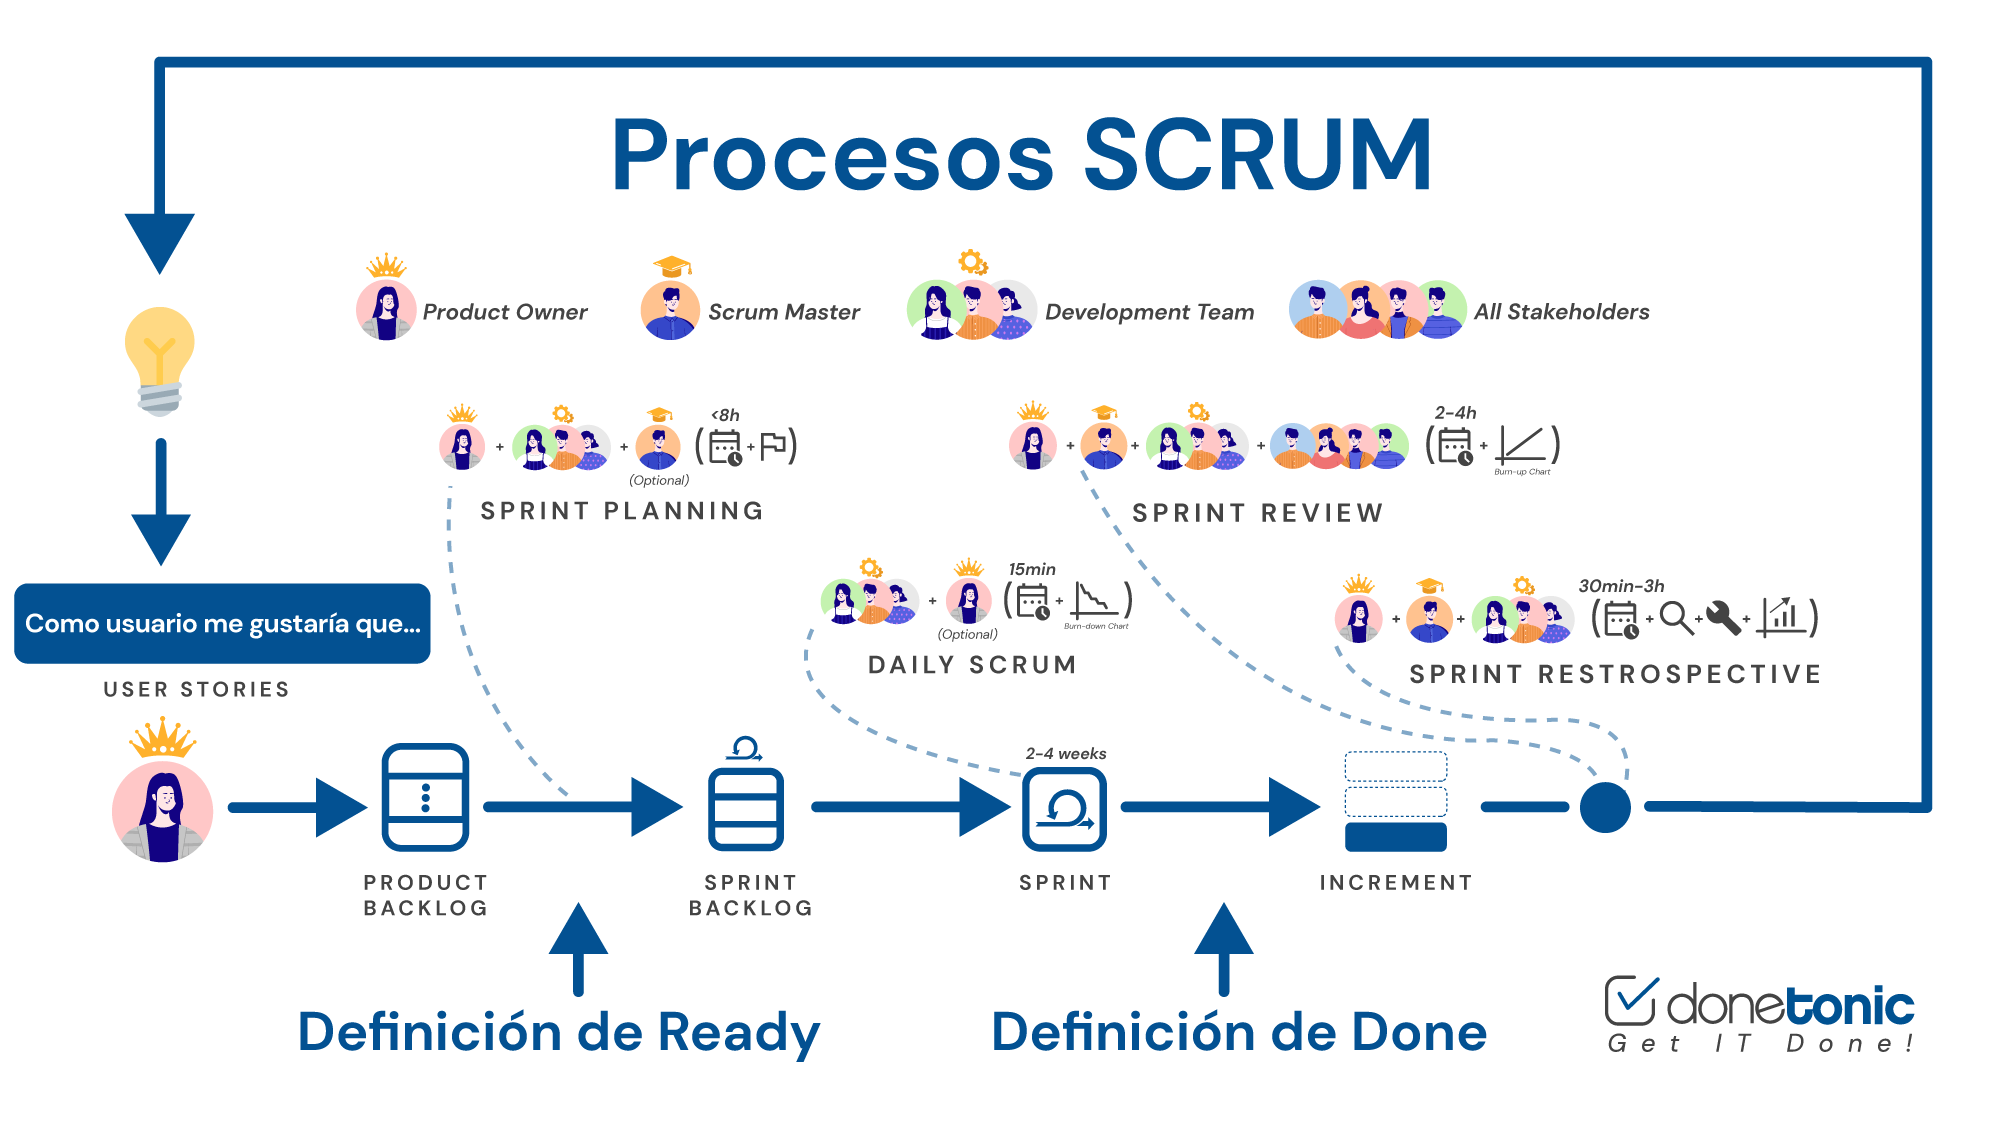
\includegraphics[scale=0.24]{imagenes/Procesos-SCRUM.png}
    \caption{Procesos SCRUM\\ Fuente: Elaboración propia}
\end{figure}

\subsection{CONCLUSIÓN}

Scrum ha demostrado ser una metodología eficaz para gestionar proyectos complejos en entornos cambiantes \autocite{sutherland2014scrum}. Su enfoque iterativo, colaborativo y centrado en el valor permite a los equipos entregar resultados de alta calidad de manera eficiente y adaptarse a los cambios del mercado. Al adoptar los roles, eventos y artefactos de Scrum, las organizaciones pueden mejorar su capacidad para gestionar proyectos y lograr sus objetivos de negocio \autocite{cohn2010suceeding}.

\section{APLICACIONES WEB}

Las aplicaciones web han emergido como un componente esencial de la infraestructura digital moderna. Estas aplicaciones, accesibles a través de navegadores web, han revolucionado la forma en que interactuamos con la información, los servicios y entre nosotros. Desde plataformas de comercio electrónico y redes sociales hasta herramientas de productividad y aplicaciones empresariales, las aplicaciones web desempeñan un papel fundamental en nuestra vida cotidiana. \citep{flanagan2011javascript}

\subsection{CARACTERÍSTICAS DE LAS APLICACIONES WEB MODERNAS}

Las aplicaciones web modernas se caracterizan por una serie de características clave que las distinguen de las aplicaciones web tradicionales:

\begin{itemize}
    \item \textbf{Interactividad:} Las aplicaciones web modernas ofrecen una experiencia de usuario altamente interactiva, similar a la de las aplicaciones de escritorio. Esto se logra mediante el uso de tecnologías como JavaScript, HTML5 y CSS3, que permiten crear interfaces de usuario dinámicas y responsivas.
    \item \textbf{Acceso a Datos en Tiempo Real:} Muchas aplicaciones web modernas se conectan a bases de datos en tiempo real para proporcionar información actualizada al instante. Esto es especialmente importante en aplicaciones como redes sociales, plataformas de trading y sistemas de monitoreo.
    \item \textbf{Escalabilidad:} Las aplicaciones web modernas están diseñadas para escalar fácilmente a medida que aumenta la demanda. Esto se logra mediante el uso de arquitecturas distribuidas y tecnologías de escalamiento horizontal, como contenedores y microservicios.
    \item \textbf{Seguridad:} La seguridad es una preocupación crítica en el desarrollo de aplicaciones web. Las aplicaciones web modernas implementan medidas de seguridad sólidas para proteger los datos de los usuarios y prevenir ataques maliciosos.
\end{itemize}

\subsection{FRONTEND Y BACKEND}

Es crucial comprender los conceptos de frontend y backend en el contexto del desarrollo web.

\subsubsection{FRONTEND}
El frontend, también conocido como "lado del cliente", se refiere a la parte de una aplicación web con la que los usuarios interactúan directamente. Incluye todo lo que el usuario ve y experimenta en su navegador, como la interfaz de usuario, los elementos visuales, la navegación y las interacciones. El desarrollo del frontend se centra en crear una experiencia de usuario atractiva, intuitiva y eficiente. \citep{basham2018developing}

\subsubsection{BACKEND}
El backend, o "lado del servidor", es la parte de una aplicación web que se ejecuta en el servidor y maneja la lógica de negocio, el acceso a datos y otras operaciones que no son visibles para el usuario. El backend se encarga de procesar las solicitudes del frontend, interactuar con bases de datos, realizar cálculos y enviar respuestas al frontend. \citep{rahman2017learning}

\subsection{STACK MERN}

El desarrollo de aplicaciones web ha experimentado una transformación radical en los últimos años, impulsada por la creciente demanda de experiencias de usuario dinámicas, interactivas y eficientes. En este contexto, el stack MERN (MongoDB, Express, React, Node.js) ha emergido como una solución poderosa y versátil para abordar estos desafíos.

\subsubsection{MONGODB}
MongoDB, una base de datos NoSQL de código abierto, se destaca por su modelo de datos flexible y escalable. A diferencia de las bases de datos relacionales tradicionales, MongoDB utiliza un modelo basado en documentos, lo que permite almacenar datos en un formato similar a JSON (BSON). Esta característica facilita la gestión de datos estructurados, semiestructurados y no estructurados, brindando una mayor agilidad en el desarrollo de aplicaciones. \citep{choquet2018mongodb}

MongoDB se caracteriza por:
\begin{itemize}
    \item \textbf{Modelo de Datos Flexible:} Utiliza un modelo de datos basado en documentos (formato BSON, similar a JSON), permitiendo almacenar datos estructurados, semiestructurados y no estructurados de manera eficiente.
    \item \textbf{Escalabilidad Horizontal:} MongoDB está diseñado para escalar horizontalmente, lo que significa que se pueden agregar más servidores a medida que crece la demanda de la aplicación.
    \item \textbf{Consultas Poderosas:} Ofrece un lenguaje de consulta rico y flexible que permite realizar búsquedas complejas y agregaciones de datos.
\end{itemize}

\subsubsection{EXPRESS}
Express, un framework web minimalista y flexible para Node.js, se ha convertido en una herramienta esencial para el desarrollo de APIs y aplicaciones web del lado del servidor. Su arquitectura modular y su amplia gama de middleware permiten a los desarrolladores construir aplicaciones personalizadas y escalables de manera eficiente. \citep{holmes2014pro}

Express simplifica el desarrollo de backend con:
\begin{itemize}
    \item \textbf{Rutas y Middleware:} Express simplifica la definición de rutas (endpoints) de la API y el uso de middleware para manejar tareas como autenticación, autorización y registro.
    \item \textbf{Minimalista y Flexible:} Express es un framework minimalista que brinda una base sólida para construir APIs personalizadas y escalables.
\end{itemize}

\subsubsection{NODE.JS}
Node.js, un entorno de ejecución de JavaScript basado en eventos, ha revolucionado el desarrollo web al permitir utilizar JavaScript tanto en el frontend como en el backend. Esta capacidad de utilizar un único lenguaje en todo el stack de desarrollo simplifica el proceso de desarrollo y fomenta la reutilización de código y habilidades. \citep{tilkov2016node}

Node.js ofrece ventajas como:
\begin{itemize}
    \item \textbf{JavaScript en el Backend:} Node.js permite utilizar JavaScript tanto en el frontend como en el backend, lo que facilita la reutilización de código y habilidades.
    \item \textbf{Eficiencia y Rendimiento:} Su arquitectura basada en eventos y no bloqueante lo hace ideal para aplicaciones en tiempo real y de alta concurrencia.
\end{itemize}

\subsubsection{NEXT.JS}
React es una libreria de JavaScript declarativa, eficiente y flexible para construir interfaces de usuario. Le permite componer interfaces de usuario complejas a partir de fragmentos de código pequeños y aislados llamados "componentes".

Next.js, un framework de React, ha ganado popularidad por su enfoque en el renderizado del lado del servidor (SSR) y su capacidad para crear aplicaciones web optimizadas para SEO y rendimiento. Next.js ofrece una serie de características que simplifican el desarrollo de aplicaciones React, como enrutamiento automático, generación de páginas estáticas y optimización de imágenes. \citep{vercel2023next}

Next.js aporta al frontend:
\begin{itemize}
    \item \textbf{Renderizado del Lado del Servidor (SSR):} Next.js ofrece SSR, mejorando el rendimiento y el SEO en comparación con el renderizado tradicional del lado del cliente (CSR).
    \item \textbf{Rutas y Enrutamiento:} Simplifica la creación de rutas y el manejo de navegación en aplicaciones React.
    \item \textbf{Optimización de Imágenes y Código:} Next.js incluye herramientas para optimizar imágenes y generar código eficiente, mejorando la velocidad de carga de la aplicación.
\end{itemize}
\section{CALIDAD Y SEGURIDAD}

El desarrollo de aplicaciones web seguras y de calidad es un desafío crucial en la era digital. La evaluación de la calidad y seguridad de estas aplicaciones requiere un enfoque integral que abarque tanto aspectos técnicos como de gestión. Las normas internacionales ISO/IEC 25000 (SQuaRE) e ISO/IEC 27034 \citep{iso25000, iso27034} brindan un marco teórico y práctico para abordar esta problemática.

\subsection{ISO/IEC 25000 (SQuaRE)}

La familia de normas ISO/IEC 25000, conocida como SQuaRE, establece un marco de referencia para la evaluación y mejora de la calidad del software \citep{iso25000}.

\subsubsection{COMPONENTES CLAVE}

\begin{itemize}
    \item \textbf{ISO/IEC 25010: Modelo de Calidad:} Define los atributos de calidad del software, como funcionalidad, fiabilidad, usabilidad, eficiencia, mantenibilidad y portabilidad.
    \item \textbf{ISO/IEC 25012: Modelo de Datos de Calidad:} Establece cómo recopilar, almacenar y analizar datos relacionados con la calidad del software.
    \item \textbf{ISO/IEC 25020: Medición de la Calidad:} Proporciona métodos para medir los atributos de calidad definidos en ISO/IEC 25010.
    \item \textbf{ISO/IEC 25040: Evaluación de la Calidad:} Ofrece un marco para evaluar la calidad del software en diferentes etapas del ciclo de vida.
\end{itemize}

\subsubsection{IMPLEMENTACIÓN}

\begin{enumerate}
    \item \textbf{Definición de Requisitos de Calidad:} Identificar los atributos de calidad más relevantes para la aplicación web y establecer los niveles de calidad deseados.
    \item \textbf{Selección de Métricas:} Elegir métricas apropiadas para medir los atributos de calidad seleccionados.
    \item \textbf{Recopilación de Datos:} Recopilar datos relevantes para las métricas seleccionadas.
    \item \textbf{Análisis de Datos:} Analizar los datos recopilados para evaluar el cumplimiento de los requisitos de calidad.
    \item \textbf{Mejora Continua:} Utilizar los resultados del análisis para identificar áreas de mejora e implementar acciones correctivas.
\end{enumerate}

\subsection{ISO/IEC 27034}

La norma ISO/IEC 27034 proporciona directrices para la seguridad de las aplicaciones a lo largo de su ciclo de vida \citep{iso27034}.

\subsubsection{COMPONENTES CLAVE}

\begin{itemize}
    \item \textbf{Gestión de Riesgos de Seguridad:} Identificar, evaluar y tratar los riesgos de seguridad en cada etapa del ciclo de vida de la aplicación.
    \item \textbf{Requisitos de Seguridad:} Definir los requisitos de seguridad para la aplicación web, teniendo en cuenta los riesgos identificados.
    \item \textbf{Diseño y Desarrollo Seguro:} Incorporar controles de seguridad en el diseño y desarrollo de la aplicación.
    \item \textbf{Pruebas de Seguridad:} Realizar pruebas de seguridad para verificar la eficacia de los controles implementados.
    \item \textbf{Operación y Mantenimiento Seguro:} Asegurar la seguridad de la aplicación durante su operación y mantenimiento.
\end{itemize}

\subsubsection{IMPLEMENTACIÓN}

\begin{enumerate}
    \item \textbf{Análisis de Riesgos:} Identificar y evaluar los riesgos de seguridad específicos para la aplicación web, utilizando técnicas como el modelado de amenazas y el análisis de vulnerabilidades.
    \item \textbf{Definición de Requisitos:} Establecer requisitos de seguridad claros y medibles para la aplicación, basados en los riesgos identificados y en las mejores prácticas de la industria.
    \item \textbf{Diseño Seguro:} Incorporar controles de seguridad en el diseño de la aplicación, como validación de entradas, autenticación y autorización, cifrado de datos y protección contra ataques comunes como inyección SQL y cross-site scripting (XSS).
    \item \textbf{Desarrollo Seguro:} Utilizar prácticas de desarrollo seguro, como revisión de código, pruebas unitarias y pruebas de seguridad estáticas y dinámicas, para detectar y corregir vulnerabilidades en el código fuente.
    \item \textbf{Implementación Segura:} Implementar la aplicación en un entorno seguro, utilizando firewalls, sistemas de detección de intrusos y otras medidas de protección, y realizar pruebas de penetración para identificar vulnerabilidades en la configuración y el despliegue.
    \item \textbf{Operación y Mantenimiento Seguro:} Monitorear la aplicación en busca de incidentes de seguridad, aplicar parches y actualizaciones de seguridad de manera oportuna, y realizar revisiones periódicas de seguridad para identificar y abordar nuevos riesgos.
\end{enumerate}

\subsection{INTEGRACIÓN DE ISO/IEC 25000 E ISO/IEC 27034}

La calidad y la seguridad son dos aspectos interrelacionados en el desarrollo de aplicaciones web. La integración de ISO/IEC 25000 e ISO/IEC 27034 permite un enfoque holístico para garantizar que la aplicación sea segura, confiable y cumpla con las expectativas de los usuarios.

\subsubsection{BENEFICIOS DE LA INTEGRACIÓN}

\begin{itemize}
    \item \textbf{Mayor seguridad:} La integración de la seguridad en el proceso de desarrollo de software desde el principio ayuda a identificar y mitigar los riesgos de seguridad de manera temprana y efectiva.
    \item \textbf{Mayor calidad:} La seguridad es un atributo de calidad esencial para las aplicaciones web. Al integrar la seguridad en el proceso de desarrollo, se mejora la calidad general de la aplicación.
    \item \textbf{Reducción de costos:} La identificación y corrección temprana de problemas de seguridad y calidad puede reducir significativamente los costos asociados con la remediación de vulnerabilidades y la resolución de incidentes de seguridad.
\end{itemize}

\subsubsection{IMPLEMENTACIÓN DE LA INTEGRACIÓN}

\begin{enumerate}
    \item \textbf{Alineación de objetivos:} Asegurar que los objetivos de calidad y seguridad estén alineados y se refuercen mutuamente.
    \item \textbf{Coordinación de actividades:} Coordinar las actividades de evaluación de calidad y seguridad para evitar duplicación de esfuerzos y maximizar la eficiencia.
    \item \textbf{Uso de herramientas integradas:} Utilizar herramientas que permitan la gestión integrada de la calidad y la seguridad, como plataformas de gestión de pruebas y herramientas de análisis de código estático.
    \item \textbf{Formación y concienciación:} Capacitar al equipo de desarrollo en las mejores prácticas de seguridad y calidad, y fomentar una cultura de seguridad y calidad en toda la organización.
\end{enumerate}


    %\input{capitulos/III-diseño-metodológico/III-diseño-metodológico}
    %\newpage
\chapter{EVALUACIÓN DE RESULTADOS}


\section{Diseño de Investigación}

\subsetction{Fase de Diseño}

\textbf{1. Objetivo del Estudio:}

   - Evaluar si una aplicación web de entrenamiento mejora el rendimiento de los estudiantes en concursos de programación competitiva tipo ICPC.
   
   - Medir el impacto en términos de porcentaje de mejora en el rendimiento.

\textbf{Preguntas de Investigación:}

   - ¿Cuál es la mejora en el rendimiento de los estudiantes después de usar la aplicación web de entrenamiento?
   
   - ¿Qué experiencias y percepciones tienen los estudiantes sobre el uso de la aplicación web?

\textbf{Hipótesis:}

   - H0: No hay una mejora significativa en el rendimiento de los estudiantes después de usar la aplicación web de entrenamiento.
   
   - H1: Hay una mejora significativa en el rendimiento de los estudiantes después de usar la aplicación web de entrenamiento.

\subsection{Fase de Recolección de Datos:}

\subsubsection{Datos Cuantitativos:}
\textbf{1. Muestra:}

   - 30 estudiantes participantes en concursos ICPC.
   
   - 15 estudiantes en el grupo experimental (uso de la aplicación).
   
   - 15 estudiantes en el grupo control (sin uso de la aplicación).

\textbf{2. Instrumentos:}

   - Pruebas de rendimiento antes y después del uso de la aplicación para ambos grupos.
   
   - Pruebas con un total de 100 puntos posibles.

\textbf{3. Procedimiento:}

   - Aplicar una prueba inicial a ambos grupos para establecer una línea base.
   
   - Implementar la aplicación web de entrenamiento durante 3 meses.
   
   - Aplicar una prueba final a ambos grupos al término del período.

   \textbf{Datos Iniciales:}
   
   - Grupo Experimental: Media de 55 puntos.
   
   - Grupo Control: Media de 54 puntos.

   \textbf{Datos Finales:}
   
   - Grupo Experimental: Media de 75 puntos.
   
   - Grupo Control: Media de 57 puntos.

\subsubsection{Datos Cualitativos:}

\textbf{1. Muestra:}

   - 10 estudiantes del grupo experimental seleccionados para entrevistas y grupos focales.

\textbf{2. Instrumentos:}

   - Guía de entrevistas semiestructuradas.
   
   - Cuestionarios de percepción y experiencia.

\textbf{3. Procedimiento:}

   - Realizar entrevistas individuales y grupos focales al final del período de uso de la aplicación.
   
   - Recoger testimonios sobre la experiencia de uso, beneficios percibidos y sugerencias de mejora.

\subsection{Fase de Análisis de Datos}

\subsubsection{Análisis Cuantitativo}


\textbf{1. Técnicas Estadísticas:}

   - Pruebas t para comparar los resultados pre y post del grupo experimental y del grupo control.
   
   - Calcular el porcentaje de mejora en los resultados.

   \textbf{Resultados:}
   
   - Grupo Experimental: Mejora media de 20 puntos (36.36\%).
   
   - Grupo Control: Mejora media de 3 puntos (5.56\%).

\textbf{2. Interpretación:}

   - Comparar los promedios de mejora entre los dos grupos.
   
   - Determinar si la mejora es estadísticamente significativa (p < 0.05).

\subsubsection{Análisis Cualitativo:}

\textbf{1. Técnicas de Análisis:}

   - Codificación de las transcripciones de entrevistas y grupos focales.
   
   - Identificación de temas y patrones emergentes.

   \textbf{Resultados:}
   
   - Temas principales: Aumento de la confianza, mejora en la comprensión de conceptos clave, percepción positiva de la usabilidad de la aplicación.

\textbf{2. Interpretación:}

   - Analizar las experiencias y percepciones de los estudiantes sobre el uso de la aplicación.
   
   - Relacionar los hallazgos cualitativos con los resultados cuantitativos para una comprensión más completa.

\subsection{Fase de Integración de Datos:}

\textbf{- Triangulación:}

  - Corroborar los hallazgos cuantitativos con las percepciones y experiencias cualitativas.
  
  - Utilizar los datos cualitativos para explicar y enriquecer los resultados cuantitativos.

  \textbf{Resultados de Triangulación:}
  
  - Los datos cuantitativos muestran una mejora significativa en el rendimiento de los estudiantes que utilizaron la aplicación web (36.36\% de mejora en el grupo experimental frente a 5.56\% en el grupo control, con p < 0.05).
  
  - Los datos cualitativos respaldan estos hallazgos, indicando que los estudiantes perciben una mejora en su comprensión de los conceptos y en su confianza para resolver problemas de programación.

\textbf{- Reporte de Resultados:}

  - Presentar los resultados cuantitativos (mejora en el rendimiento) junto con las narrativas cualitativas (experiencias y percepciones).
  
  - Discutir la implicación de los hallazgos y proporcionar recomendaciones para la implementación y mejora de la aplicación web.

  \textbf{Reporte Final:}
  
  - Los estudiantes que utilizaron la aplicación web de entrenamiento mostraron una mejora significativa en su rendimiento en las pruebas de programación, lo que respalda la hipótesis de que dicha aplicación puede ser una herramienta efectiva para mejorar el rendimiento en concursos tipo ICPC.
  
  - Las experiencias y percepciones de los estudiantes resaltan la usabilidad y efectividad de la aplicación, sugiriendo que su diseño y contenido son adecuados para el entrenamiento en programación competitiva.

\begin{markdown}
## Implementación del Estudio

1. **Preparación:**
   - **Desarrollo y Validación de Pruebas de Rendimiento:** Se desarrollaron dos pruebas de rendimiento de programación competitiva, cada una con un total de 100 puntos posibles. Las pruebas fueron validadas por expertos en programación competitiva.
   - **Diseño y Pilotaje de Entrevistas y Cuestionarios:** Se diseñó una guía de entrevistas semiestructuradas y un cuestionario de percepción y experiencia. Ambos instrumentos fueron pilotados con un grupo pequeño de estudiantes para asegurar su claridad y relevancia.
   - **Selección y Preparación de los Participantes:** Se seleccionaron 50 estudiantes participantes en concursos ICPC y se dividieron aleatoriamente en dos grupos: grupo experimental (25 estudiantes) y grupo control (25 estudiantes).

2. **Ejecución:**
   - **Pruebas Iniciales:**
     - Grupo Experimental: Media de 55 puntos (Desviación estándar: 10).
     - Grupo Control: Media de 54 puntos (Desviación estándar: 9).
   - **Implementación de la Aplicación Web:** El grupo experimental utilizó la aplicación web de entrenamiento durante 3 meses, con un mínimo de 2 horas de uso por semana.
   - **Supervisión y Apoyo:** Se proporcionó soporte técnico y tutorías semanales para asegurar el uso adecuado de la aplicación.
   - **Pruebas Finales:**
     - Grupo Experimental: Media de 75 puntos (Desviación estándar: 8).
     - Grupo Control: Media de 57 puntos (Desviación estándar: 7).

3. **Recolección de Datos:**
   - **Resultados de las Pruebas de Rendimiento:**
     - **Grupo Experimental:** Mejora media de 20 puntos (36.36%).
     - **Grupo Control:** Mejora media de 3 puntos (5.56%).
   - **Entrevistas y Grupos Focales:**
     - Se realizaron entrevistas semiestructuradas con 10 estudiantes del grupo experimental.
     - Se llevaron a cabo 2 grupos focales con los mismos estudiantes para profundizar en sus experiencias y percepciones.

4. **Análisis:**
   - **Análisis Cuantitativo:**
     - **Pruebas t para muestras relacionadas:**
       - Grupo Experimental: t(24) = 8.23, p < 0.001.
       - Grupo Control: t(24) = 1.57, p = 0.13.
     - **Interpretación:** La mejora en el grupo experimental fue significativa, mientras que en el grupo control no se encontró una mejora significativa.
   - **Análisis Cualitativo:**
     - **Codificación y Temas Emergentes:**
       - Aumento de la confianza en la resolución de problemas.
       - Mejora en la comprensión de conceptos clave de programación.
       - Percepción positiva de la usabilidad y efectividad de la aplicación.
     - **Citas Representativas:**
       - "La aplicación me ayudó a entender mejor los algoritmos que siempre me costaban."
       - "Me siento más seguro en los concursos después de usar la aplicación."

5. **Integración y Reporte de Resultados:**
   - **Triangulación:**
     - Los datos cuantitativos mostraron una mejora significativa en el rendimiento de los estudiantes del grupo experimental (36.36% de mejora) comparado con el grupo control (5.56% de mejora), con p < 0.001.
     - Los datos cualitativos respaldaron estos hallazgos, indicando que los estudiantes perciben una mejora en su comprensión de los conceptos y en su confianza para resolver problemas de programación.
   - **Reporte de Resultados:**
     - Los estudiantes que utilizaron la aplicación web de entrenamiento mostraron una mejora significativa en su rendimiento en las pruebas de programación, lo que respalda la hipótesis de que dicha aplicación puede ser una herramienta efectiva para mejorar el rendimiento en concursos tipo ICPC.
     - Las experiencias y percepciones de los estudiantes resaltan la usabilidad y efectividad de la aplicación, sugiriendo que su diseño y contenido son adecuados para el entrenamiento en programación competitiva.

## Conclusión
El estudio sugiere que el desarrollo y uso de una aplicación web de entrenamiento puede mejorar significativamente el rendimiento de los estudiantes en concursos de programación competitiva del tipo ICPC. Los datos cuantitativos y cualitativos combinados proporcionan una comprensión integral de los beneficios de la aplicación, destacando tanto la mejora en el rendimiento como las experiencias positivas de los estudiantes.
\end{markdown}






%\section{ESTUDIO DE CASO}
%\section{INVENTARIO DE LOS RESULTADOS}


% Titulo tentativo
%\section{ESTUDIO DE CASO}
%\section{INVENTARIO DE LOS RESULTADOS}
%    \subsection{ENCUESTAS PREPARADAS PARA LA POBLACIÓN DE ESTUDIANTES ANTES DE REALIZAR LA PLATAFORMA}
%    \subsection{ENCUESTA PARA LA POBLACIÓN DE CONCURSANTES DE LA ICPC}
%    \section{ENCUESTA PREPARADAS PARA USUARIOS CON EXPERIENCIA EN CONCURSOS DE PROGRAMACIÓN.}
%\section{RESULTADOS ALCANZADOS}

    %\newpage
\chapter{BIBLIOGRAFÍA}

\printbibliography


%[heading=none]
    %\chapter{ANEXOS}
    \section{CRONOGRAMA}

    \begin{figure}[H]
        \centering
        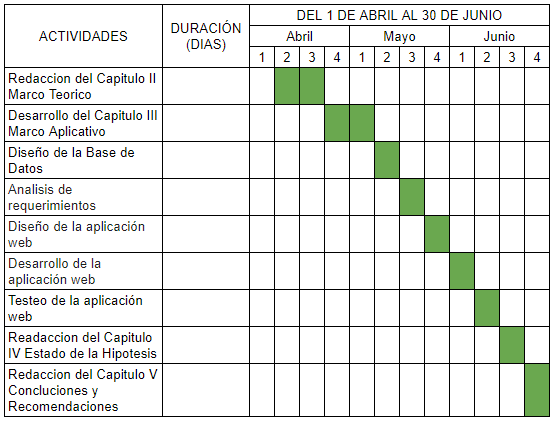
\includegraphics[scale=1.2]{imagenes/cronograma-2024.png}
        %\caption{\\ Fuente: \citep{icpc-glogal}}
    \end{figure}
    
        
    % \endgroup
    % \bibliographystyle{apacite}
    % \bibliography{capitulos/biblio.bib}
	%--------------------------------------------------
	
	
	
	%BACKMATTER
	%---------------------------------------------------
% 	\backmatter
% 	%BIBLIOGRAFÍA.
% 	%\cleardoublepage
% 	\addcontentsline{toc}{chapter}{Bibliografía}
% 	\bibliographystyle{apalike}
% 		\bibliography{capitulos/biblio}
		
	%---------------------------------------------------	
	
\end{document}


%NO OLVIDAR CITAR!